\section{Escaping mediocrity in the well-specified scenario}

As a starting point, we consider the well-specified case of $p=1$. As we are going to see, this case captures almost all of the phenomenology of interest, and is helpful to build an intuition for how SGD escapes mediocrity. Moreover, despite its apparent simplicity, this case has been the subject of several works in the literature \citep{sun2016geometric,tan2019online,chen2019gradient,arous2021online}. In particular, \cite{chen2019gradient} established a convergence rate $t=O(\log{d})$ for randomly initialized gradient descent on the population risk. In our setting \eqref{2305:eq:sgd}, this corresponds to the $\gamma\to 0^{+}$ limit, and translates to a sample complexity of $n=O(d\log{d})$. \cite{tan2019online} provided a refined analysis that accounts for the stochasticity in one-pass SGD, reaching a similar $n=O(d\log{d})$ rate for escaping mediocrity, in agreement with the general information exponent characterization of \cite{arous2021online}. 

In this section, we show that in the high-dimensional limit, the sample complexity constant for one-pass SGD can be well estimated from the deterministic reduction \eqref{2305:eq:def:overlap_process}. In particular, we show that the stochastic corrections from a finer analysis of the process \eqref{2305:eq:def:overlap_process} can be neglected. 

\subsection{Population risk landscape}
% \begin{figure}
%     \centering
%     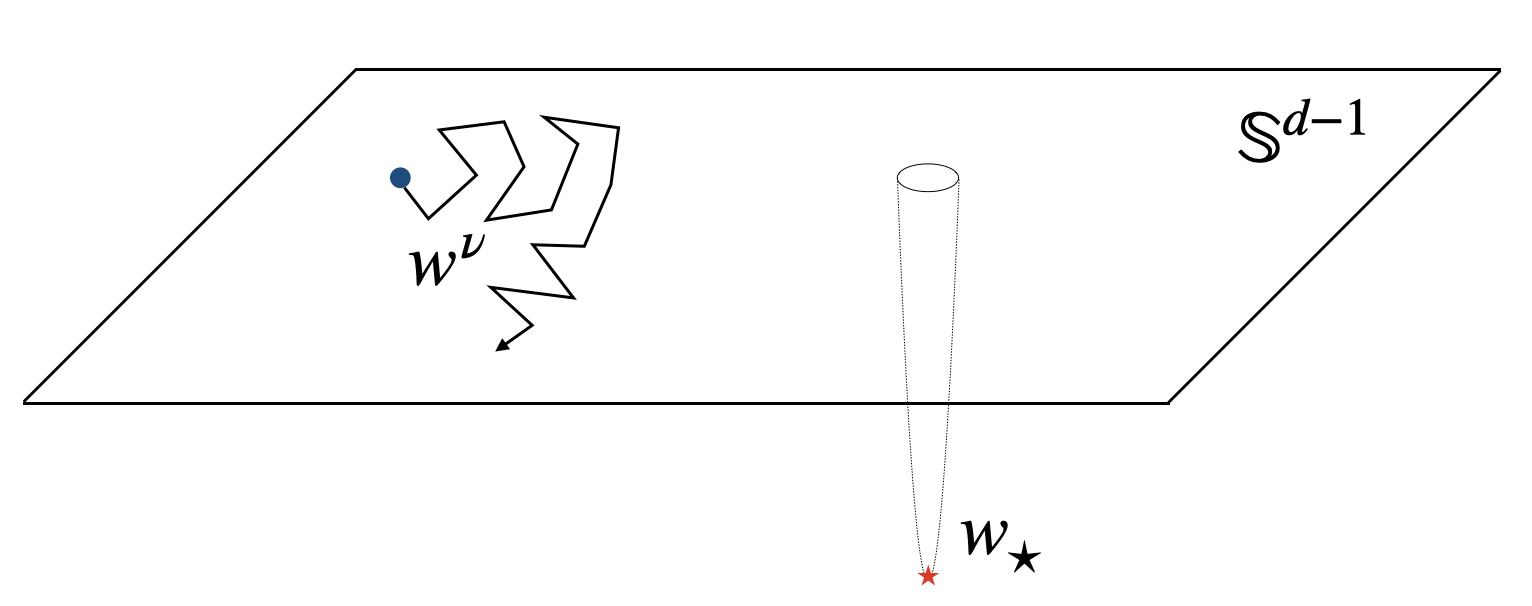
\includegraphics[width=0.8\textwidth]{figs/landscape}
%     \caption{Low-dimensional illustration of mediocrity at initialization. As discussed in Sec. \ref{2305:sec:app:spherical}, the expected Hessian at initialization is a strict saddle-point with $d-1$ flat directions and a single negative direction pointing towards the global minimum. This scenario is particularly hard for descent based algorithms such as SGD, that require $n=d\log{d}$ samples / steps to develop significant correlation with the signal.}
%     \label{2305:fig:app:landscape}
% \end{figure}
As previously discussed, one-pass stochastic gradient descent can be seen as a discretisation of gradient flow on the population risk \cite{robbins1951stochastic}. Therefore, understanding the geometry of the population risk can provide useful insight into the behaviour of SGD. For $p=1$ and imposing the spherical constraint, the population risk \eqref{2305:eq:def:risk} considerably simplifies since everything can be expressed in terms of a single, scalar sufficient statistics $m =\sfrac{1}{d} w_{\star}^{\top}w\in[-1,1]$:
\begin{align}
    \mathcal{R}(w) - \frac{\Delta}{2} = 2(1-m^2)
\end{align}
From this expression, it is easy to see that we have two global minima $m=\pm 1$ (corresponding to $w=\pm w_{\star}$) and one global maximum $m=0$ (corresponding to $w\perp w_{\star}$). Indeed, the spherical gradient of the population risk can also be computed explicitly (see Appendix \ref{2305:sec:app:spherical} for details):
\begin{align}
   {\rm grad}_{\mathbb{S}^{d-1}}\mathcal{R}(w) = 4m\left(m w-w_{\star}\right)
\end{align}
 which confirm that these are the only critical points. Finally, we can also compute the spherical Hessian exactly: 
\begin{align}
 {\rm Hess}_{\mathcal{S}^{d-1}}\mathcal{R}(w) = 4\left[m^2 I_{d}+m w w_{\star}^{\top}-w_{\star}w_{\star}^{\top}\right]
\end{align}
Note that for $w=\pm w_{\star}$ $(m=\pm 1)$ the Hessian is proportional to the identity, hence positive definite as expected for a minimum. Instead, for $w \perp w_{\star}$ $(m=0)$, the Hessian becomes a rank-one matrix with $d-1$ zero eigenvalues and a single negative eigenvalue with eigenvector proportional to $w_{\star}$. Hence, $m=0$ also corresponds to a \emph{strict saddle}, i.e. the landscape is flat along most of the directions, except for one that points towards the signal. Note that with high probability, we have precisely $m\approx 0$ for an uninformed random initialisation in high-dimensions $d\to\infty$.

This provides a typical picture of mediocrity in high-dimensions, where the landscape resembles a flat golf course with a single hole, see Fig. \ref{2305:fig:app:landscape}.

\subsection{Exit time from deterministic limit}
\label{2305:sec:exit:deterministic}
We now move to the description of the one-pass SGD dynamics. Our key goal in this section is to determine how much data / how long SGD takes in order to find the signal in the high-dimensional limit $d\to\infty$. As we have discussed in Section \ref{2305:sec:odes}, in this limit the sufficient statistics concentrate, with its evolution being described by the following deterministic ODE:
\begin{align} \label{2305:eq:spherical-p1-ode}
  \dod{\bar{m}{(t)}}{t} &= \bar{m}{(t)}\left[4(1-6\gamma)(1-\bar{m}^2{(t)})-2\gamma\Delta\right]\quad\text{with}\quad
  \bar{m}(t)\in[-1,1]
\end{align}
 with initial condition $\bar{m}(0)=\sfrac{1}{d}w_{\star}^{\top}w^{0}$. See Appendix \ref{2305:app:spherical_constraint} for an explicit derivation. Figure \ref{2305:fig:sde_p1} (left) compares the evolution of the risk predicted from solving the high-dimensional ODEs \eqref{2305:eq:spherical-p1-ode} with different finite size ($d=3000$) simulated instances of the problem, showing a a good agreement between the theory and the averaged population risk over the different runs. 

Given the spherical constraint, the population risk is now simply given by $\risk{(m)} = 2 \left(1-m^2\right)+\sfrac{\Delta}{2}$. From this expression, it is clear that $m=\pm 1$ are global minima and $m=0$ is a global maximum. Therefore, the information theoretically minimum achievable risk is $\mathcal{R}(\pm 1) = \min \mathcal{R}(m) = \sfrac{\Delta}{2}$. 

We start with two immediate observations that can be drawn from \eqref{2305:eq:spherical-p1-ode}. First, we have a necessary upper bound on the learning rate for learning to occur: \(\lr < \sfrac{1}{6}\). Moreover, from fixed-point stability analysis we can get the value where \(\bar{m}\) converges for large times, and, consequently, the asymptotic excess population risk achievable in this setting is:
\begin{equation}
  \lim_{t\to\infty}\risk(\bar{m}(t))-\sfrac{\Delta}{2} = \frac{\gamma\Delta}{1-6\gamma}.
\end{equation}
The presence of an asymptotic risk plateau for the excess risk is consistent with previous results for the high-dimensional limit of two-layers neural networks \citep{saad1996dynamics,goldt2019dynamics}. Note that in the population gradient flow limit $\gamma\to 0^{+}$, SGD converges to the minimal risk \cite{robbins1951stochastic}. Indeed, the presence of a finite excess risk even in the well-specified setting is an intrinsic correction from the SGD noise in the high-dimensional regime where $\sfrac{1}{d}\ll \gamma$ \citep{veiga2022phase}, and can be related to the radius of the asymptotic stationary distribution of the weights around the global minima \citep{pflug1986stochastic,dieuleveut2020bridging}.


We now move to our main problem: estimating the time SGD takes to escape mediocrity at initialization. Let $T\in[0,1]$ be the relative difference with respect to the initial value of the risk, and let \(t_\text{ext}\) be the time when the risk exits the region above the threshold \(T\), see Fig. \ref{2305:fig:sde_p1} (right) for an illustration. By construction, \(t_\text{ext}\) can be found by solving the following equation:
\begin{equation} \label{2305:eq:exit_time_implicit_equation}
  (1-T)\left(\risk{\left(\bar{m}(0)\right)}-\frac{\Delta}{2}\right) = \left(\risk\left({\bar{m}\left(t_\text{ext}\right)}\right)-\frac{\Delta}{2}\right).
\end{equation}
The above can be exactly solved by numerically integrating \eqref{2305:eq:spherical-p1-ode} and then finding the root of \eqref{2305:eq:exit_time_implicit_equation}. However, an analytical expression for the ODE exit time can be found from the following two observations:
\begin{itemize}
    \item From the discussion around equation ~\eqref{2305:eq:initial_distribution_QM}, initializing at random in high-dimensions imply that \(\bar{m}(0)=\varepsilon \ll 1\), so we can consider the linearization of equation \eqref{2305:eq:spherical-p1-ode} in $\varepsilon$ and solve it analytically. For small enough \(T\), this will lead us to an accurate result;
    \item Even if the ODE trajectories are deterministic, the exit time \(t_\text{ext}\) is a random variable of the random initialization.
\end{itemize}
Note there these lead to two natural notions of average exit time over the initial conditions. The first one is obtained by taking the expected value over initial conditions before solving the cross-threshold equation
\begin{equation}\label{2305:eq:exit_time_p1}
    t_\text{ext}^\text{(anl)} = \frac{\log\left[Td+(1-T)\right]}{8(1-6\gamma)-4\gamma\Delta}.
\end{equation}
Borrowing the jargon from statistical physics, we refer to $t_\text{ext}^\text{(anl)}$ as the \emph{annealed exit time}. The second option is to take the expected value exit time obtained from solving \eqref{2305:eq:spherical-p1-ode} over a fixed initial condition:
\begin{equation}
\label{2305:eq:exit:quenched}
    t_\text{ext}^\text{(qnc)} = \mathbb E_{\mu_0 \sim \chi^2(1)} \left[
        \frac{\log\left[\frac{Td}{\mu_0}+(1-T)\right]}{8(1-6\gamma)-4\gamma\Delta)}
    \right].
\end{equation}
Again, borrowing the jargon from statistical physics we refer to $t_\text{ext}^\text{(qnc)}$ as the \emph{quenched exit time}. Some comments on this result are in order:
\begin{itemize}
    \item By concavity of the logarithm function, we have $t^{\rm (qnc)}_{\rm ext}\geq t^{\rm (anl)}_{\rm ext}$.
    \item For both notions, we have $t_{\rm ext} = O(\log{d})$ implying $n=O(d\log{d})$ samples are required to escape mediocrity, consistent with the rates in the literature \citep{chen2019gradient,tan2019online,arous2021online}.
    \item Both exit times are monotonically increasing in both $\gamma\in[0,\sfrac{1}{6}]$ and $\Delta\geq 0$. Recalling that $\delta t = \sfrac{\gamma}{d}$, this implies the existence of an optimal learning rate $\gamma_{\rm opt}=\sfrac{1}{(12+\Delta)}$ that minimizes the number of samples required to escape mediocrity.
\end{itemize}

\subsection{Does stochasticity matters?} \label{2305:sec:sde_p1}
Note that the initial correlation parameter at random initialization \eqref{2305:eq:initial_conditions_unconstrainted} is given by:
\begin{align}
    m^{0} = O(\sfrac{1}{\sqrt{d}})
\end{align}
Therefore, in the high-dimensional limit $d\to\infty$ in which the ODE description \eqref{2305:eq:spherical-p1-ode} is exact, we have $\bar{m}(0) = 0$. This is a fixed point \eqref{2305:eq:spherical-p1-ode}, which suggests that that strictly in the high-dimensional limit SGD is trapped forever at mediocrity. However, in practice we always have $d<\infty$, meaning that at initialization we always have a non-zero correlation with the signal $m^{0}=\varepsilon \ll 1$. Moreover, at high but finite dimensions, \eqref{2305:eq:spherical-p1-ode} is just an approximation to the actual stochastic dynamics \eqref{2305:eq:def:overlap_process}. Indeed, this is precisely what we used in order to estimate the exit time from the deterministic ODE \eqref{2305:eq:spherical-p1-ode}. While the stochastic corrections to the high-dimensional limit does not radically change the convergence rate scaling \citep{tan2019online} (and hence the mediocrity picture), it is important to ask whether it leads to important corrections on the precise exit time. 

Stochastic corrections to the deterministic high-dimensional limit of one-pass SGD have been recently discussed in a broad setting by \cite{arous2022high}. In particular, this work has shown that close to a fixed point the the process for the sufficient statistics \eqref{2305:eq:def:overlap_process} can be well approximated in the high-dimensional limit by a diffusion process with drift potential given by the corresponding deterministic ODEs. We follow a similar strategy, and consider the following process specilezed in the case \(p=1\):
% The main idea is noting that in Eqs.~\eqref{2305:eq:overlapping_ODE} the ODEs are obtained as the expected value of some random variables, and thus we can add some perturbation as noise computed from their covariance matrix.
% Focusing on the unconstrained case with \(p=1\), we can evolve Eqs.~\eqref{2305:eq:overlapping_ODE} in a stochastic differential equation
\begin{equation}\label{2305:eq:overlapping_SDE}
    \begin{split}
    \dif \M_{1} &= \Psi_{1}{(\Omega)}\dif t + \sqrt{\frac{\gamma}{d}}   \vec{\sigma}_\M{(\Omega)} \cdot \dif \b_t \\
    \dif \Q_{11} &= \Phi_{11}{(\Omega)}\dif t + \sqrt{\frac{\gamma}{d}}   \vec{\sigma}_\Q{(\Omega)} \cdot \dif \b_t 
    \end{split}
\end{equation}
where \(\dif \b_t\) is a 2-dimensional Wiener process, and \(\vec{\sigma}_M\) and \(\vec{\sigma}_Q\) are defined as
\begin{equation}
    \begin{pmatrix}
    \vec{\sigma}_\M\\
    \vec{\sigma}_\Q
  \end{pmatrix}
  \coloneqq
  \sqrt{
    \begin{pmatrix}
        \Var_{(\lf,\lf_\star)\sim\mathcal{N}(0_{\hids+1}, \Omega)}{\left[\mathcal{M}_1\right]} &
        \Cov_{(\lf,\lf_\star)\sim\mathcal{N}(0_{\hids+1}, \Omega)}{\left[\mathcal{M}_1,\mathcal{Q}_{11}\right]} \\
        \Cov_{(\lf,\lf_\star)\sim\mathcal{N}(0_{\hids+1}, \Omega)}{\left[\mathcal{M}_1,\mathcal{Q}_{11}\right]} &
        \Var_{(\lf,\lf_\star)\sim\mathcal{N}(0_{\hids+1}, \Omega)}{\left[\mathcal{Q}_{11}\right]}
    \end{pmatrix}
  }.
\end{equation}
\begin{figure}
    \centering
    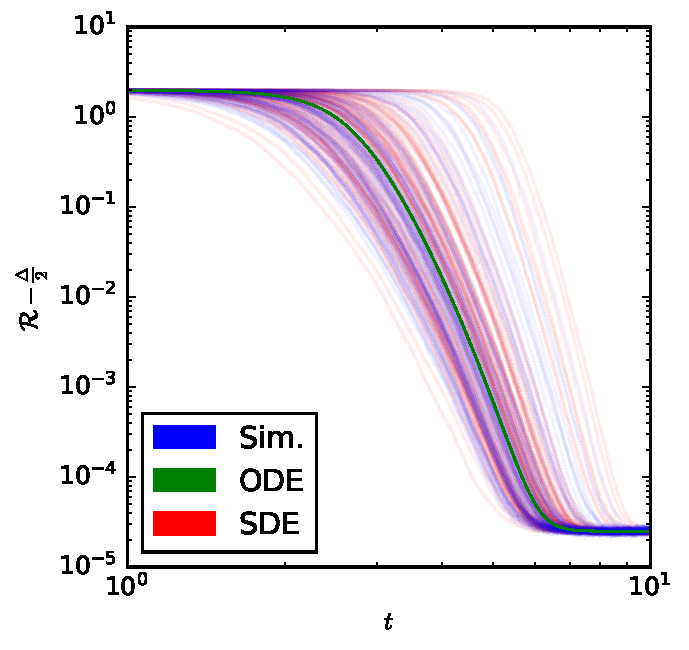
\includegraphics[width=0.49\textwidth]{figs/sde_example}
    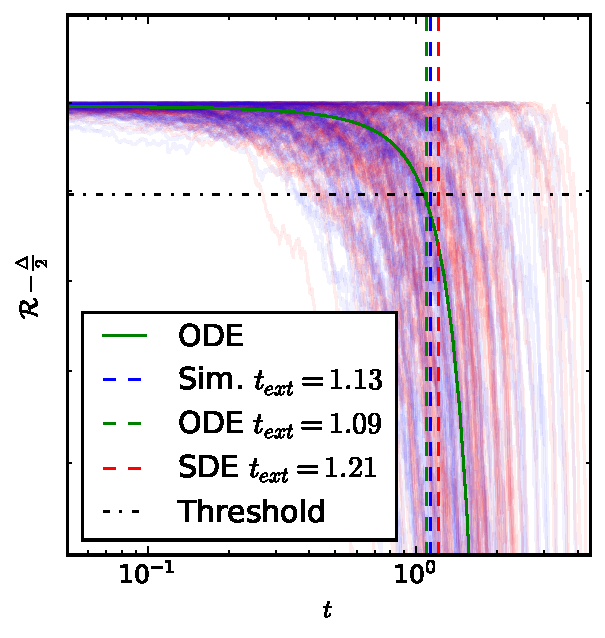
\includegraphics[width=0.43\textwidth]{figs/sde_example-zoom}
    \caption{multiple run of the simulated SGD and the numerically integrated SDE, always starting from the same initial condition, with \(d=3000\).
    All the \(t_\text{ext}\) presented are obtained by solving numerically \eqref{2305:eq:exit_time_implicit_equation}.
    The SDE captures the variance that the ODE doesn't exhibit, but the $t_\text{ext}$ do not change considerably.}
    \label{2305:fig:sde_p1}
\end{figure}
The stochastic corrections are analogous with the ones obtained by \cite{arous2022high}; in Appendix~\ref{2305:app:match_with_GBA} we present an alternative derivation of them, following their approch, and we highlight the fact that our formulae generalize their result.
Notice that the stochastic correction is proportional to \(\sqrt{\sfrac{\gamma}{d}}\), consistent to a first order correction to the deterministic limit. Similarly to the discussion in Section \ref{2305:sec:exit:deterministic}, the spherical constraint can be imposed by projecting the process in the sphere. This is discussed in detail in App.~\ref{2305:app:spherical_constraint}, and for $p=1$ reads:
\begin{equation}
\label{2305:eq:sde:p1}
\begin{split}
 \dod{\M_1}{t} &= \left(\Psi_{1}{(\mat{\Omega})} - \frac{\M_{1}}{2}\Phi_{11}{(\mat{\Omega})}\right)\dif t + \sqrt{\frac{\gamma}{d}}   \left(\vec{\sigma}_\M-\frac{m_1}{2}\vec{\sigma}_\Q\right)\cdot\dif\b_t 
\end{split}
\end{equation}
Figure~\ref{2305:fig:sde_p1} compares different instances of finite size simulations with instances of the SDE \eqref{2305:eq:sde:p1} with the same initial condition. Although the stochastic correction offers a better description of the process at large but finite dimensions, we find that quite surprisingly they have a small impact in the exit time. Hence, the formulas \eqref{2305:eq:exit_time_p1} \& \eqref{2305:eq:exit:quenched} derived in the Section \ref{2305:sec:exit:deterministic} for random initialization provide a good approximation to the exit time. In Appendix ~\ref{2305:app:SDE_exit_time} we discuss how to derive an exit time formulae with the stochastic corrections, both annealed and quenched one. As just showed, the new formulas do not offer any improvements compared to the deterministic ones, nevertheless the stochastic process can describe the dynamic even when the initialization is exactly \(m=0\), that is a fixed point of the ODE.

To summarize, in this section we have shown that the deterministic ODEs provides a good approximation for the precise number of samples required for escaping mediocrity in high-dimensions. In other words, stochasticity \emph{does not help} in navigating the flat directions at initalization and correlating with the signal.


% %%%%%%%%%%%%%%%%%%%%%%%%%%%%%%%%%%%%%%%%%%%%%%%%%%%%%%%%%%%%%%%%%%%%%%%%%%%%%%%
